\documentclass[12pt, a4paper]{article}
\usepackage[utf8]{inputenc}
% \usepackage{pdflscape}
\usepackage{rotating}
% \usepackage{lscape}
\usepackage{amssymb}
\usepackage{indentfirst}
\usepackage{listings}
\usepackage{enumitem}
\usepackage{comment}
\usepackage{graphicx}
\usepackage{color}
\usepackage[portuguese]{babel}
\usepackage{geometry}
\geometry{legalpaper, a4paper,
 total={170mm,257mm},
 left=20mm,
 top=20mm}
\setlength{\voffset}{-10mm}
\definecolor{dkgreen}{rgb}{0,0.6,0}
\definecolor{gray}{rgb}{0.5,0.5,0.5}
\definecolor{mauve}{rgb}{0.58,0,0.82}

\lstset{frame=tb,
  language=Java,
  aboveskip=3mm,
  belowskip=3mm,
  showstringspaces=false,
  columns=flexible,
  basicstyle={\small\ttfamily},
  numbers=none,
  numberstyle=\tiny\color{gray},
  keywordstyle=\color{blue},
  commentstyle=\color{dkgreen},
  stringstyle=\color{mauve},
  breaklines=true,
  breakatwhitespace=true,
  tabsize=3
}

\newcommand{\tit}[1]{\textit{#1}}
\newcommand{\tb}[1]{\textbf{#1}}
\newcommand{\tbi}[1]{\textbf{\textit{#1}}}

\newcommand{\bitem}[2]{ \tb{(\tit{#1}) {#2}}}
\newcommand{\iitem}[1]{(\tit{#1})}

\newcommand{\oo}{orientação à objetos}
\newcommand{\sw}{\tit{software}}
\newcommand{\ssw}{\tit{software} }

\newcommand{\question}[1]{\item \tb{#1}}
\newcommand{\answer}[1]{\par \tb{Resposta:} #1}

\newcommand{\quotes}[1]{``#1''}

\title{Módulo 6 - Atividade Individual \\
  \large Diagrama de Sequência}

\author{Wellington M. Espindula}
\date{Maio de 2021}

\begin{document}
    \maketitle
    
    \begin{enumerate}[label=\textbf{\arabic*.}]
        % Question 1
        \question{Banco. Crie o diagrama de sequência.
            \normalfont{\tit{Um cliente informa ao funcionário de um banco o número da conta que deverá receber o valor a ser depositado. O funcionário em resposta verificará se essa conta existe, solicitando sua consulta à interface do sistema; esta repassará o número da conta ao controlador que, em resposta, disparará o método consultar\_Conta. Se a conta informada for encontrada, o funcionário solicitará o valor a ser depositado e o cliente o fornecerá. O funcionário então informará à interface do sistema a quantidade do valor a depositar. Esse valor será repassado ao controlador, que disparará o método depositar\_valor. Se esse método for realizado com sucesso, o controlador pedirá à interface que apresente uma mensagem informando que a operação foi concluída.}}
        }
        \answer{
          \begin{figure}[!ht]
              \centering
              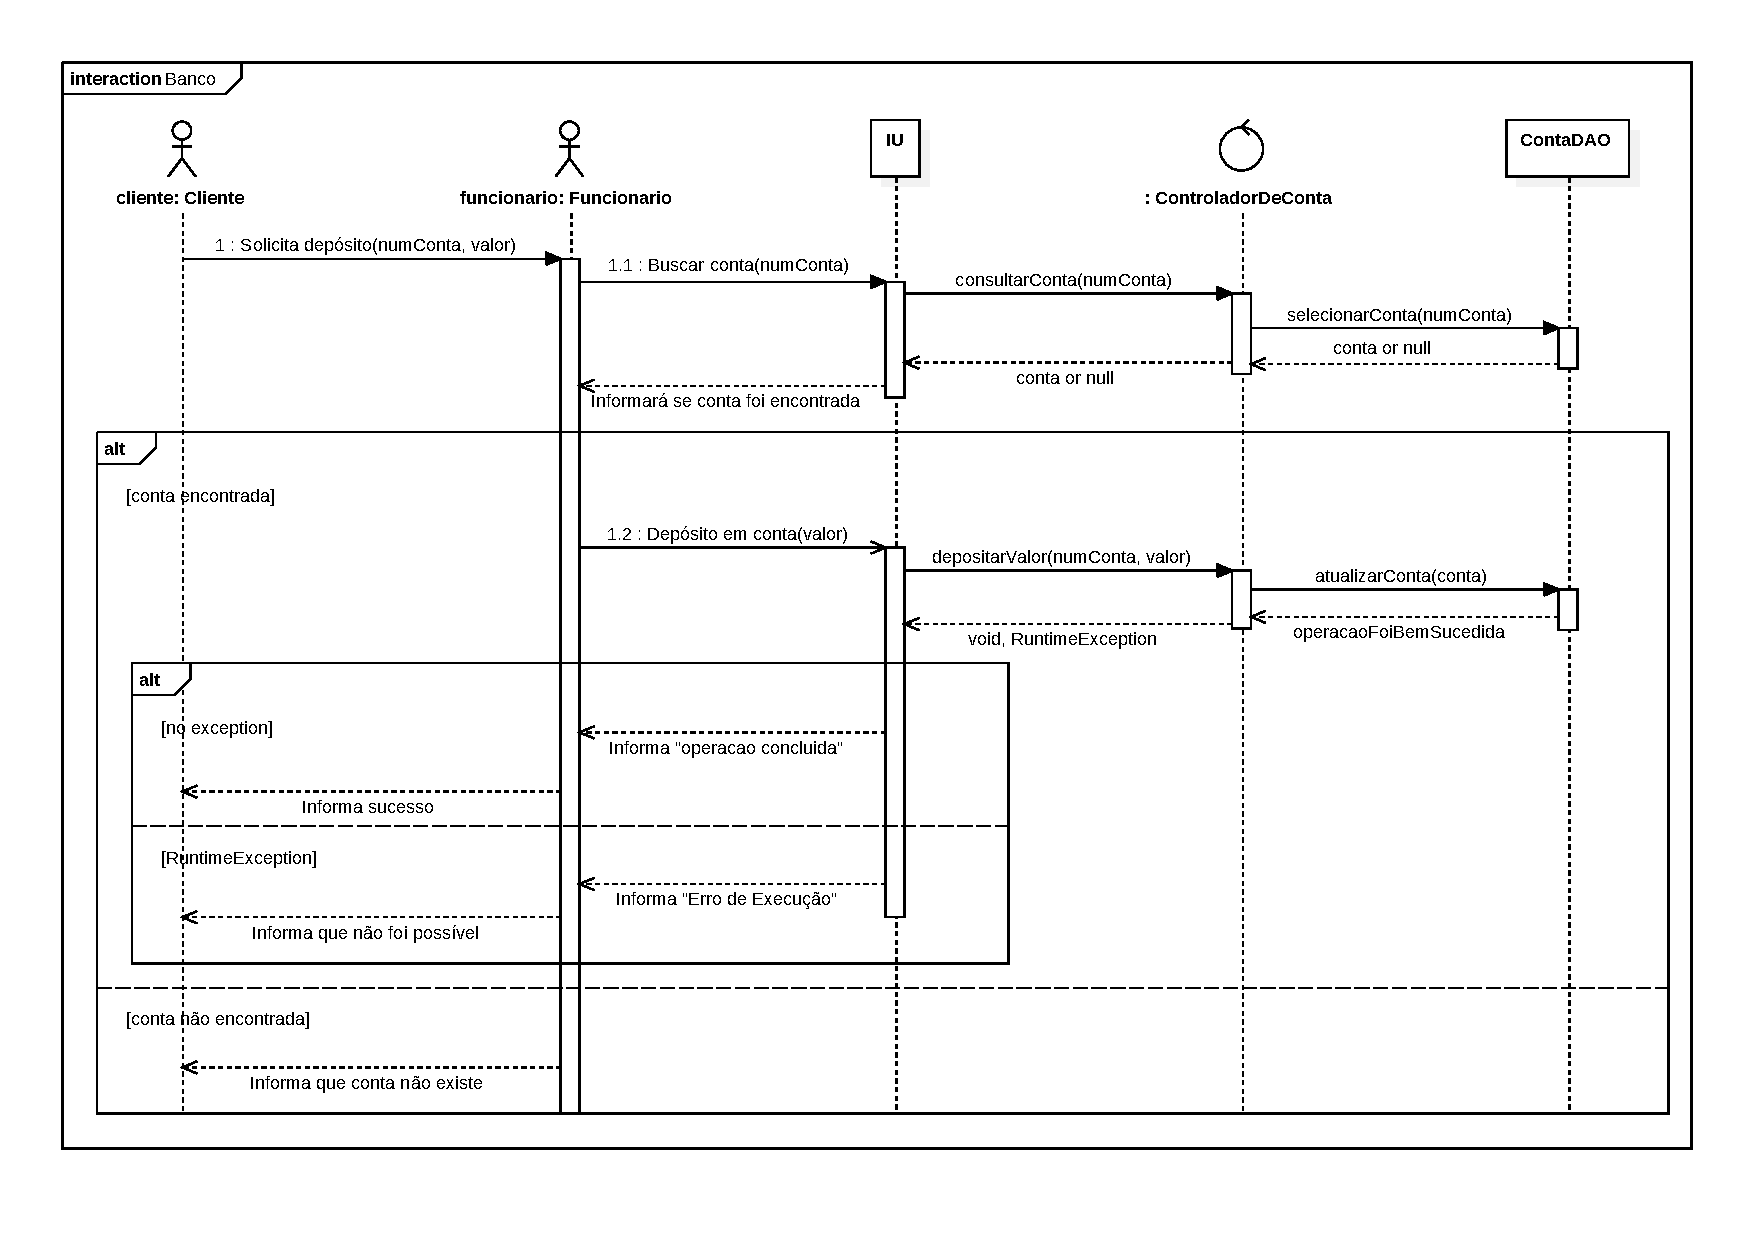
\includegraphics[width=\textwidth]{q1.pdf}
                \caption{Diagrama de Sequência do Banco. Fonte: O Autor, 2021.}
              \label{fig:question1}
          \end{figure}
        } \newpage
        
        % Question 2
        \question{WebShop. Considere uma loja web que possui os componentes mostrados no diagrama UML a seguir. Desenhe um diagrama de sequência para este caso de uso.}
        \answer{
          \begin{figure}[!ht]
              \centering
              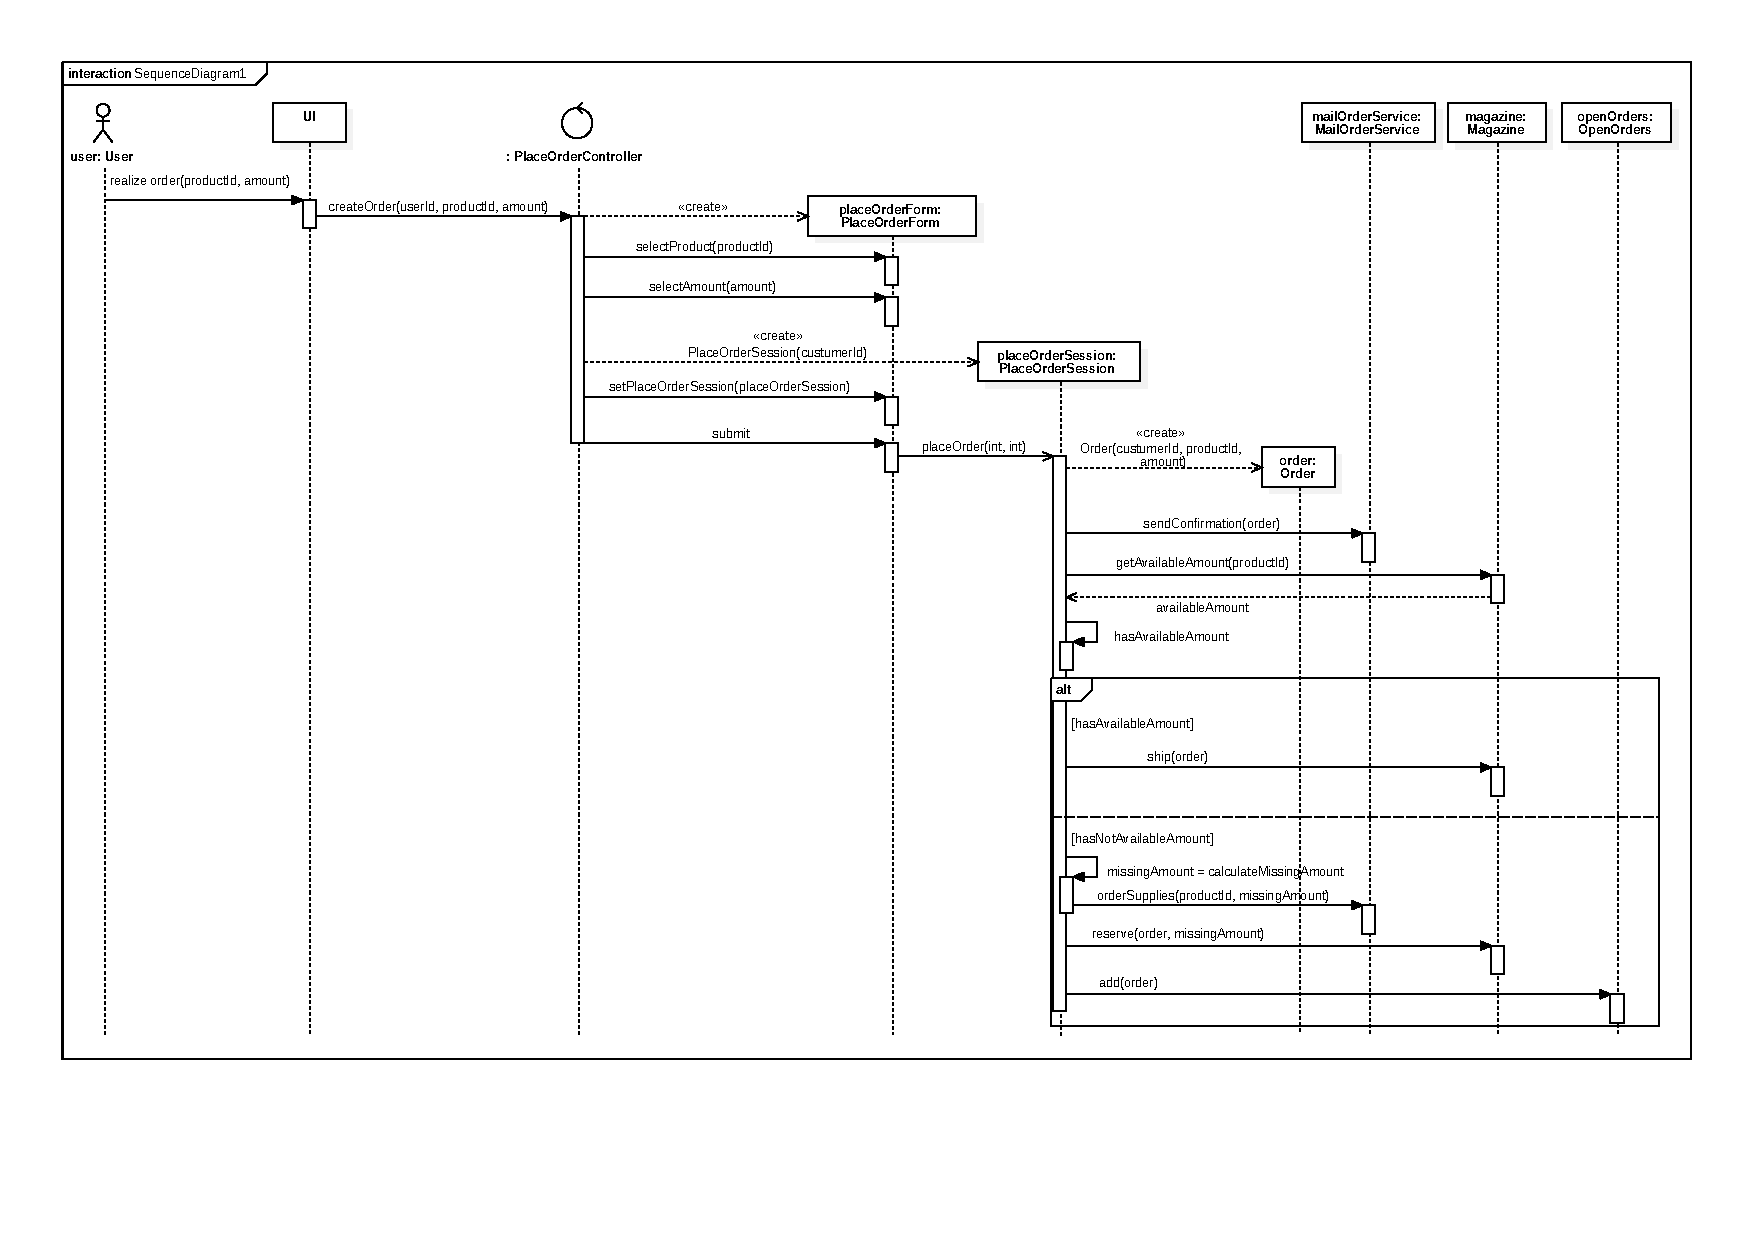
\includegraphics[width=\textwidth]{q2.pdf}
                \caption{Diagrama de Sequência do WebShop. Fonte: O Autor, 2021.}
              \label{fig:question2}
          \end{figure}
        } \newpage
        
        % Question 3
        \question{
            Sistema de Biblioteca. \normalfont{Com base no enunciado do sistema da biblioteca e demais artefatos fornecidos (incluindo o modelo conceitual e descrições de caso de uso), faça o projeto detalhado do caso de uso “Efetuar empréstimo”, representando-o com um diagrama de classes e diagrama de sequência.}
        }
        \answer{
         \begin{figure}[!ht]
              \centering
              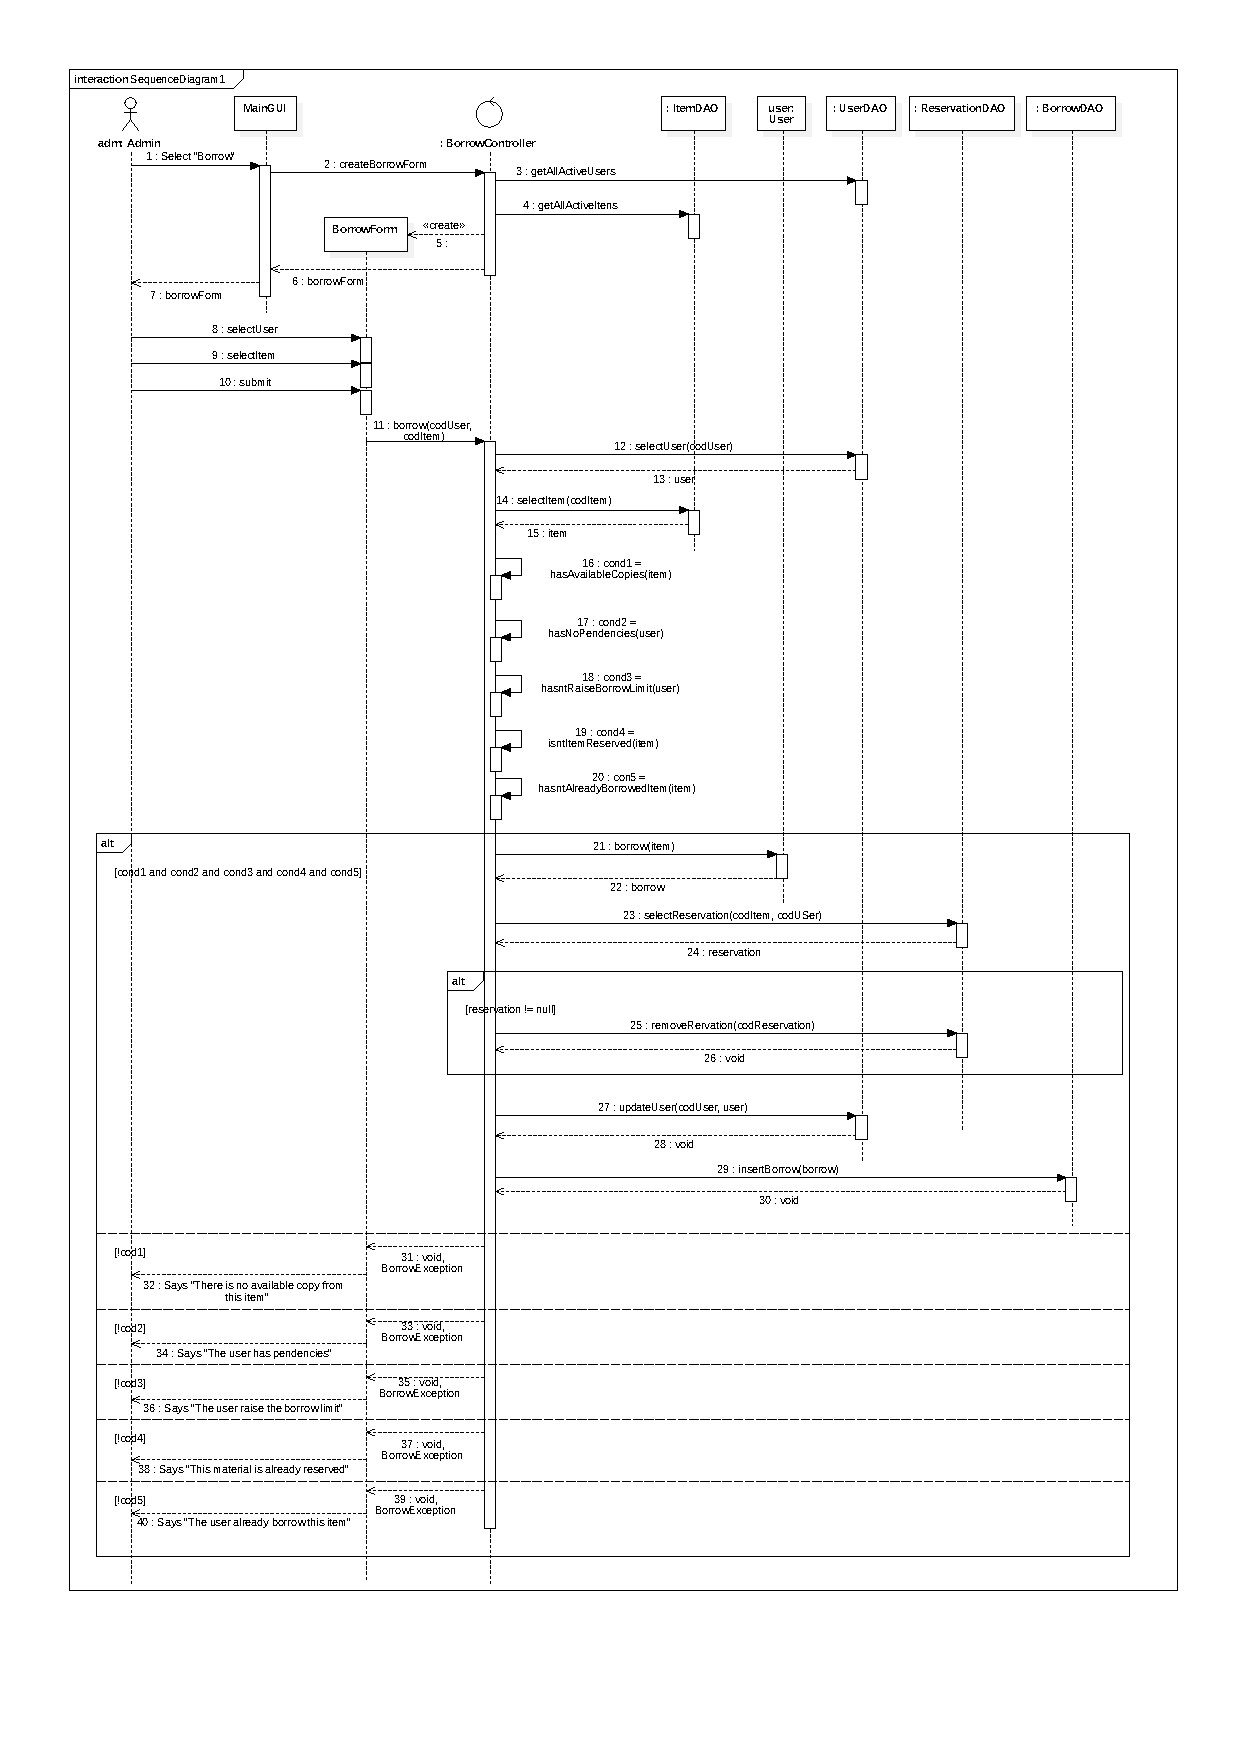
\includegraphics[height=0.82\textheight]{q3.pdf}
                \caption{Diagrama de Sequência do Sistema Biblioteca. Fonte: O Autor, 2021.}
              \label{fig:question3}
          \end{figure}
        }
        \newpage
        
        % Question 4
        \question{Sistema de Assistência Pré-natal. \normalfont{Com base nos artefatos fornecidos sobre o sistema de assistência pré-natal (diagrama de casos de uso e descrição de um caso de uso), fazer o projeto arquitetural do sistema (representando-o com uma notação adequada) e o projeto detalhado do caso de uso “Realizar consulta” (representando-o com um diagrama de classes e diagrama de sequência). A arquitetura do sistema pode estar de acordo com as seguintes alternativas: (i) com uma base de dados central e acessado por aplicações-clientes instaladas nos diversos computadores do hospital; ou (ii) com um servidor central que é acessado por navegadores web instalados nos diversos computadores do hospital.}}
        \answer{ 
         \begin{figure}[!ht]
              \centering
              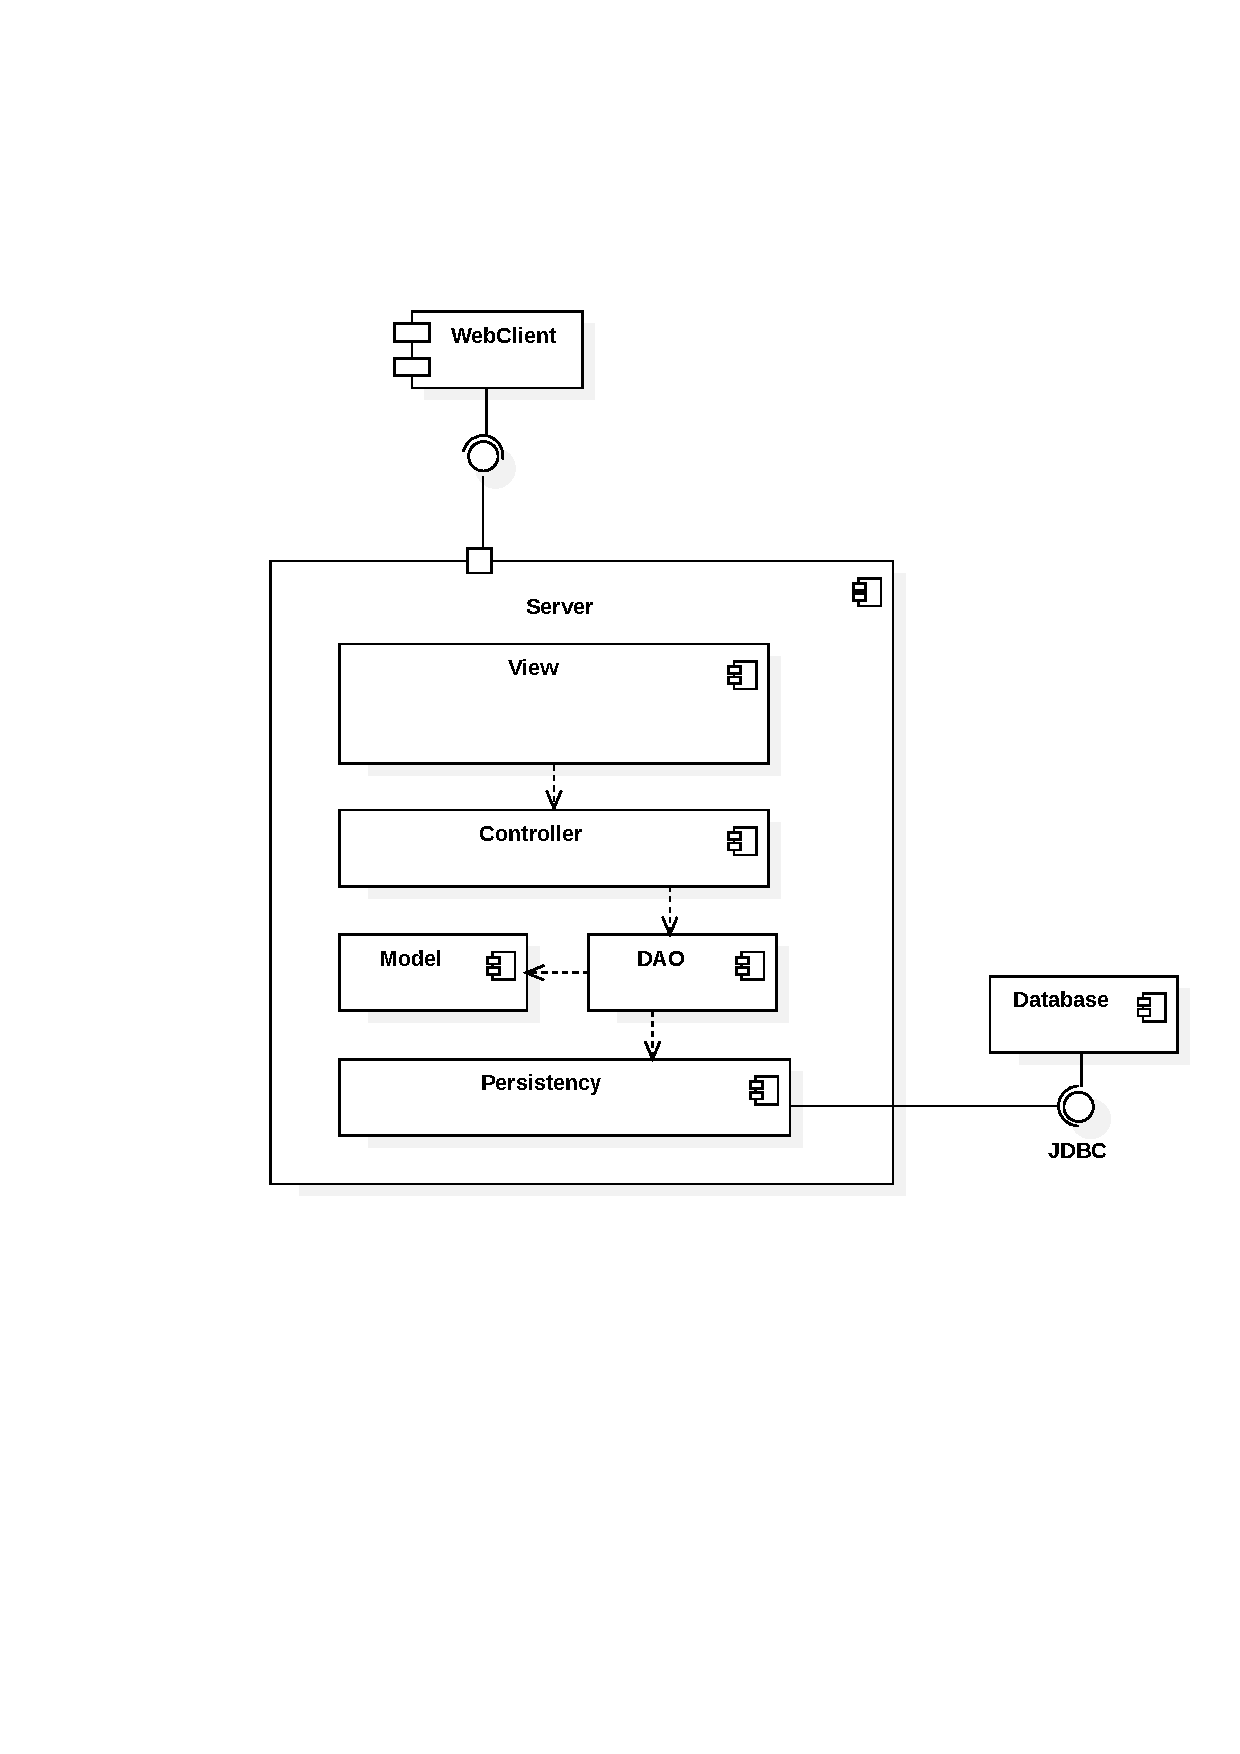
\includegraphics[height=0.4\textheight, trim = 4cm 9cm 1cm 5cm, clip]{q4a.pdf}
                \caption{Diagrama de Componentes Caso do Sistema de Assistência Pré-natal. Fonte: O Autor, 2021.}
              \label{fig:question4a}
          \end{figure}         
         
        \begin{figure}[!ht]
              \centering
              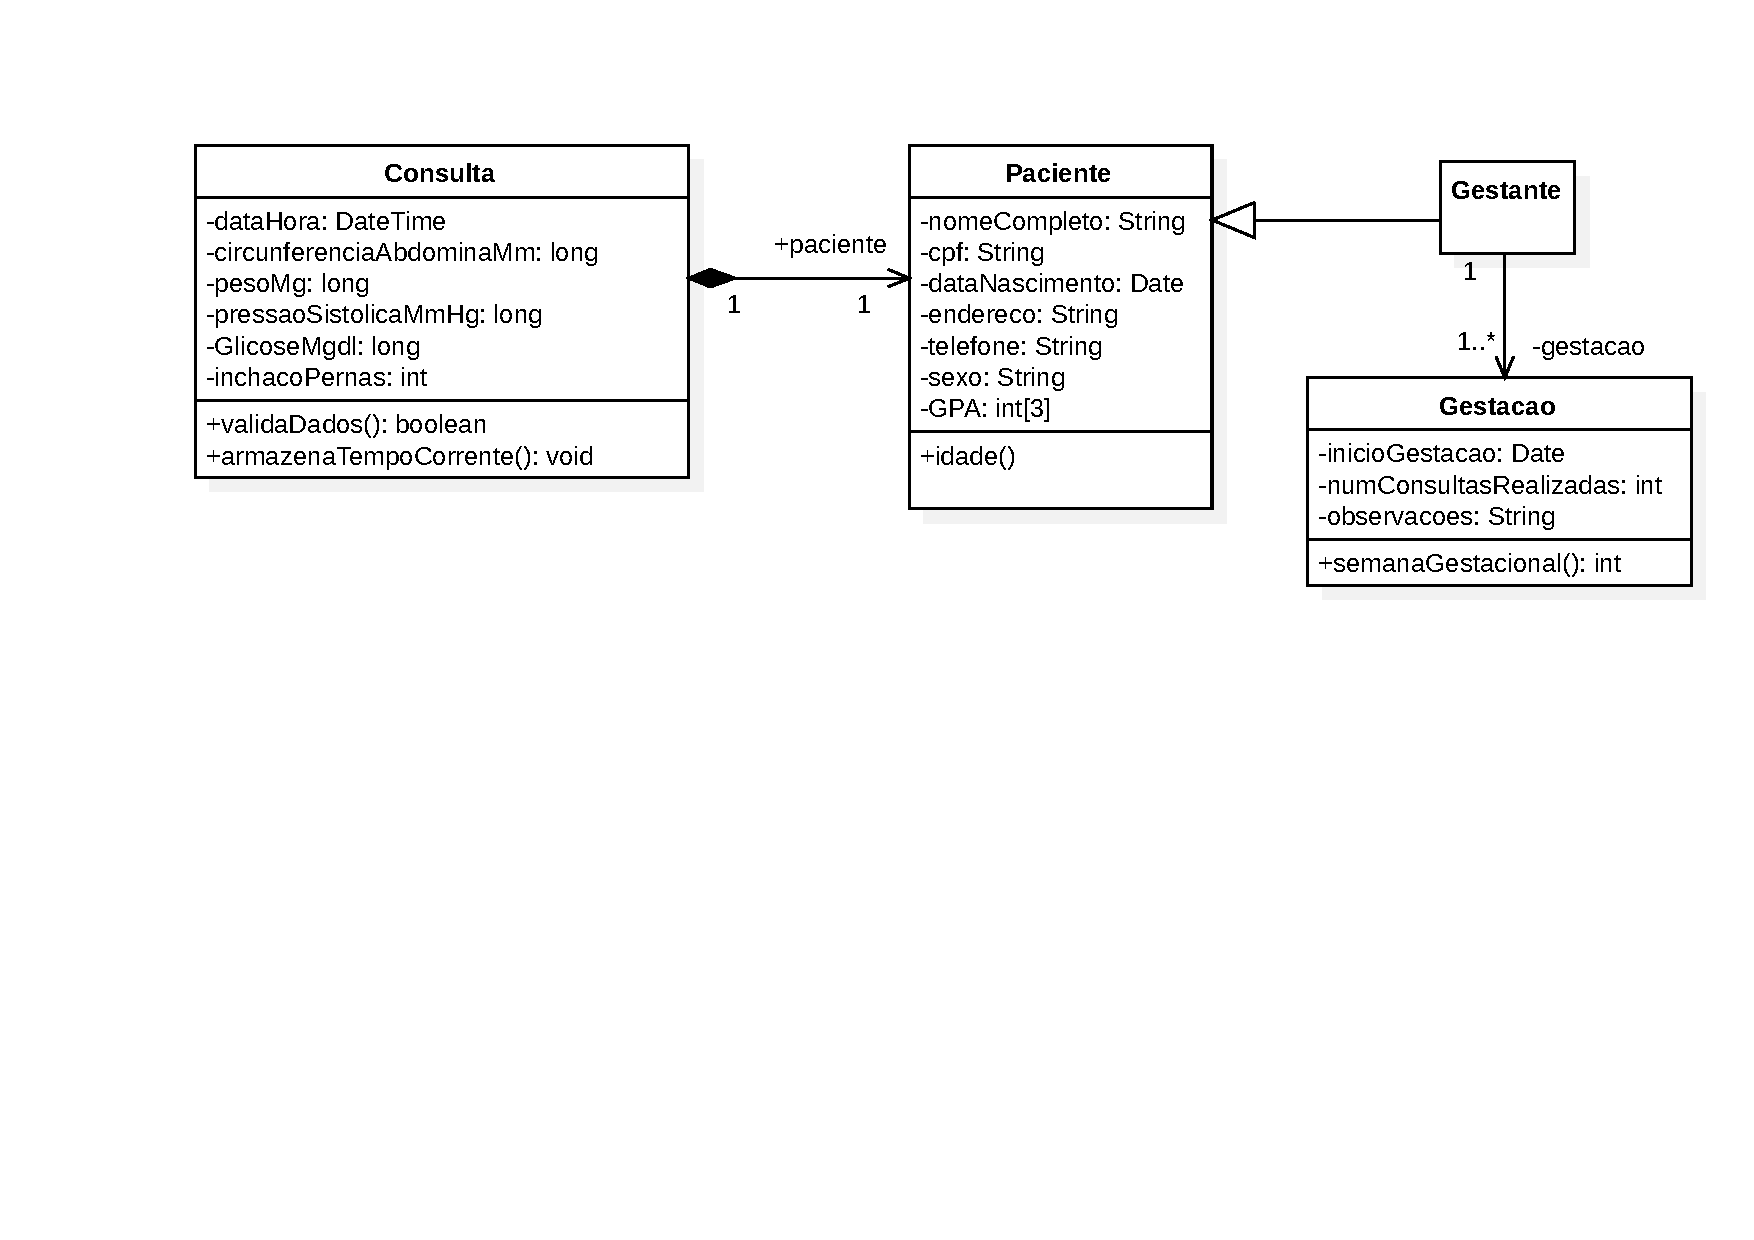
\includegraphics[width=\textwidth, trim = 3cm 11cm 1cm 2cm, clip]{q4b.pdf}
                \caption{Diagrama de Classes do Caso de Uso Realiza Consulta. Fonte: O Autor, 2021.}
              \label{fig:question4b}
          \end{figure}         
          
        %   \newpage
        %   \begin{landscape}
              \begin{sidewaysfigure}[!ht]
                  \centering
                  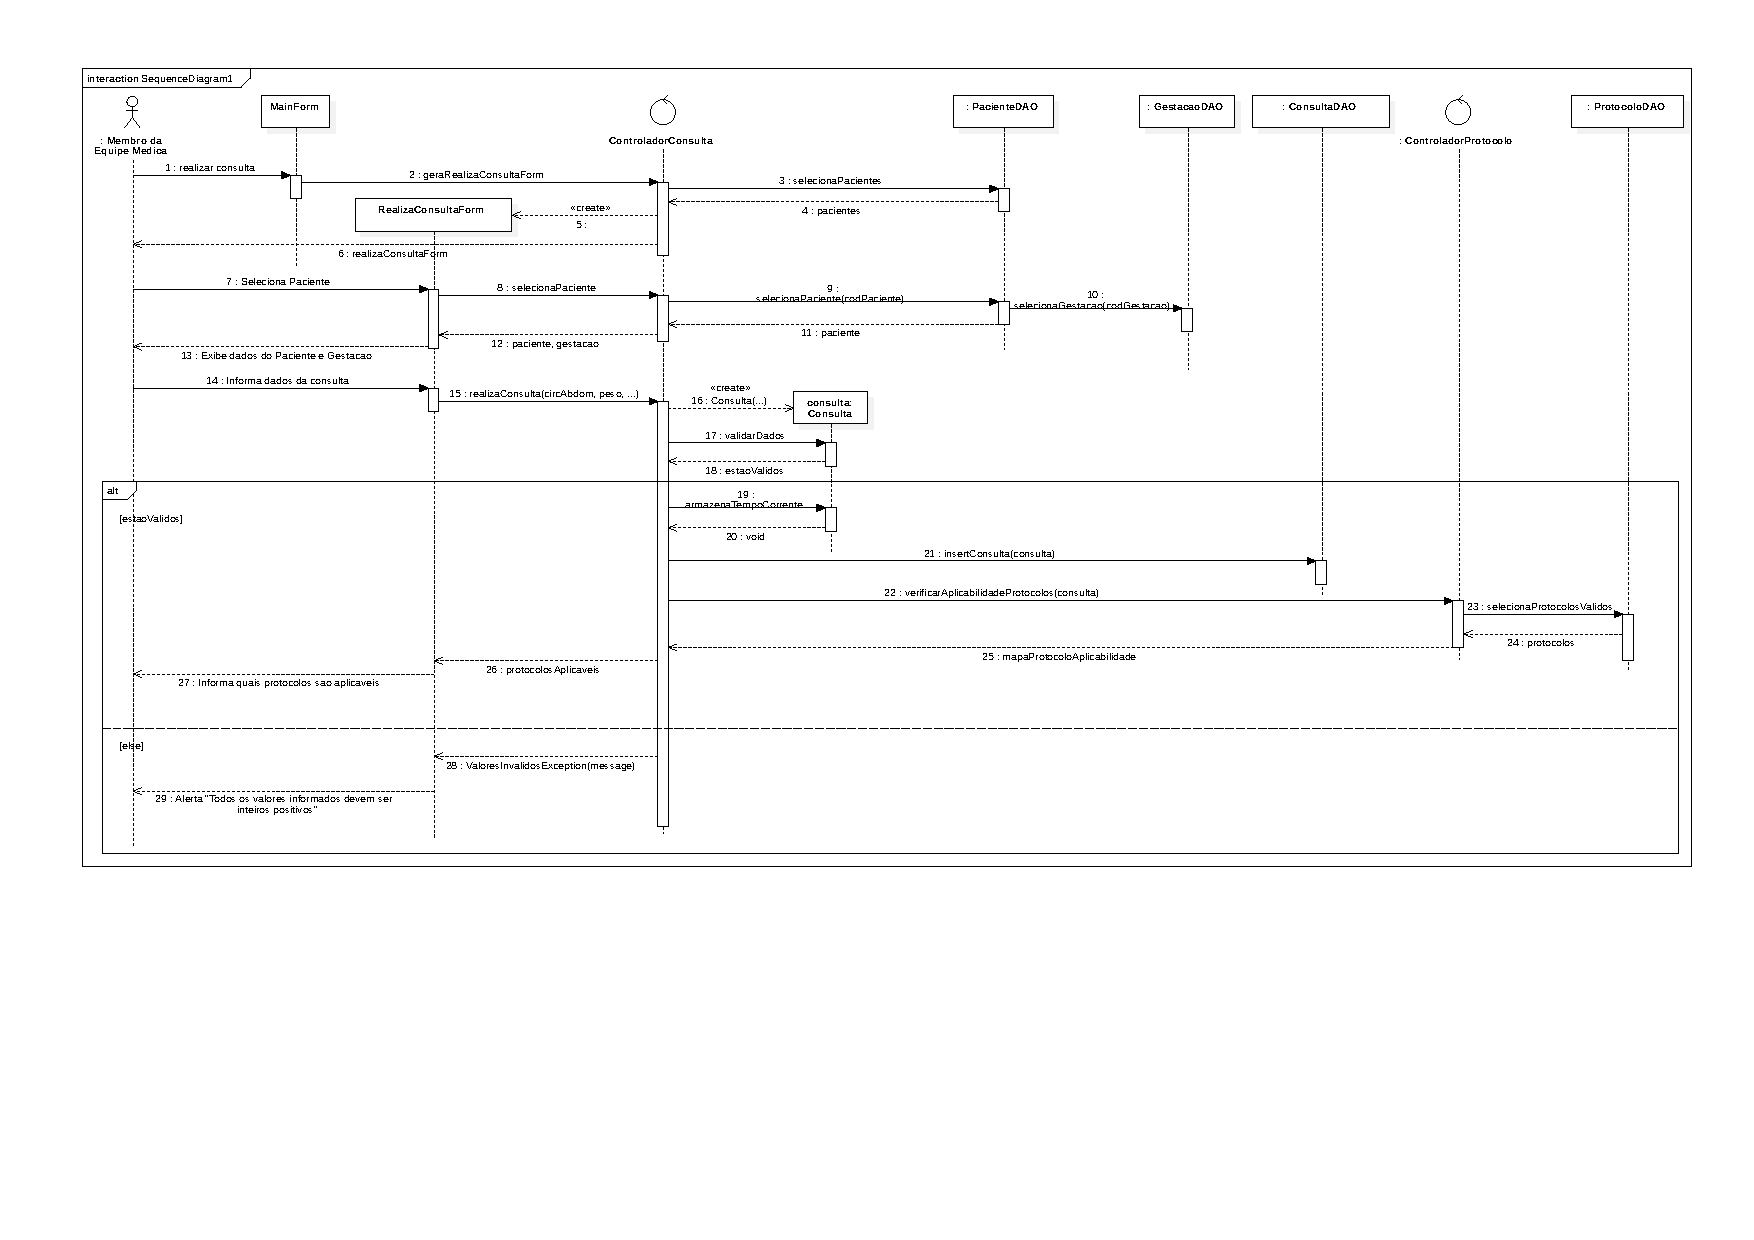
\includegraphics[width=\textwidth, trim = 1cm 6cm 0cm 1cm, clip]{q4c.pdf}
                    \caption{Diagrama de Sequência do Caso de Uso Realiza Consulta. Fonte: O Autor, 2021.}
                  \label{fig:question4c}
              \end{sidewaysfigure}
        %   \end{landscape}

         \clearpage
            Dados os diagramas \ref{fig:question4a}, \ref{fig:question4b} e \ref{fig:question4c}, pode-se notar a presença do padrão Controlador - um dos 5 padrões do GRASP. Utilizei-o dado que era necessário uma classe que realizassem o controle dos eventos de interação com o usuário, removendo a lógica de tratamento de eventos da interface de usuário ou das classes de domínio; por conseguinte, reduzindo a dependência direta entre a interface de usuário, persistência e classes de domínio e também mantendo as classes coesas.
        }
       
    
    \end{enumerate}
        
    
\end{document}